\section{Johdanto}

Kielimalli on autoregressiivinen malli, joka ennustaa seuraavan sanan (tai tokenin) aiemman kontekstin perusteella. Kun mallin tuottama sana liitetään aiempaan kontekstiin, voidaan kutsua mallia päivitetyllä kontekstilla ja näin malli voi tuottaa pitkiäkin tekstijaksoja. Suuret kielimallit ovat viime vuosina kehittyneet pelkistä tekstin tuottajista järjestelmiksi, jotka kykenevät myös hyödyntämään ulkoisia työkaluja.  Jos kielimallia suorittava ympäristö tulkitsee tiettyjä mallin tuottamia merkintöjä työkalukutsuina, kielimalli voi käyttää esimerkiksi laskentaa, verkkohakua tai tietokantakyselyitä.

Luonnollisen kielen käyttö tietokantojen rajapintana on kiinnostava sovelluskohde, koska se voi madaltaa datan hyödyntämisen kynnystä. Tällöin käyttäjän ei tarvitse osata SQL-kieltä eikä tuntea tietokannan rakennetta yksityiskohtaisesti, vaan hän voi esittää tiedontarpeensa tavallisella kielellä. Käytännön hyöty riippuu kuitenkin siitä, kuinka luotettavasti järjestelmä kykenee tulkitsemaan käyttäjän tarkoituksen ja muuntamaan sen oikeaksi SQL-kyselyksi.

Tässä tutkielmassa tarkastellaan Snowflaken Cortex Analyst -järjestelmää tapaustutkimuksena. Cortex Analyst on kielimallipohjainen työkalu, joka muodostaa käyttäjän luonnollisen kielen kysymyksistä SQL-kyselyitä ja voi suorittaa niitä tietokantaa vasten. Tutkimuskohteena on puhelinkeskusdataa sisältävä tietokanta, jossa analyysin keskiössä on yksi keskusteludataa sisältävä päätason taulu sekä kolme sitä täydentävää taulua (ks. kuva \ref{fig:table_spec}). Järjestelmän toiminta perustuu semanttiseen näkymään, jossa taulut, kentät ja niiden merkitykset kuvataan YAML-muodossa (ks. kuva \ref{fig:example_semantic_view}). Tämä näkymä toimii linkkinä käyttäjän luonnollisen kielen kysymyksen ja tietokannan rakenteen välillä.

\begin{figure}
  \centering
  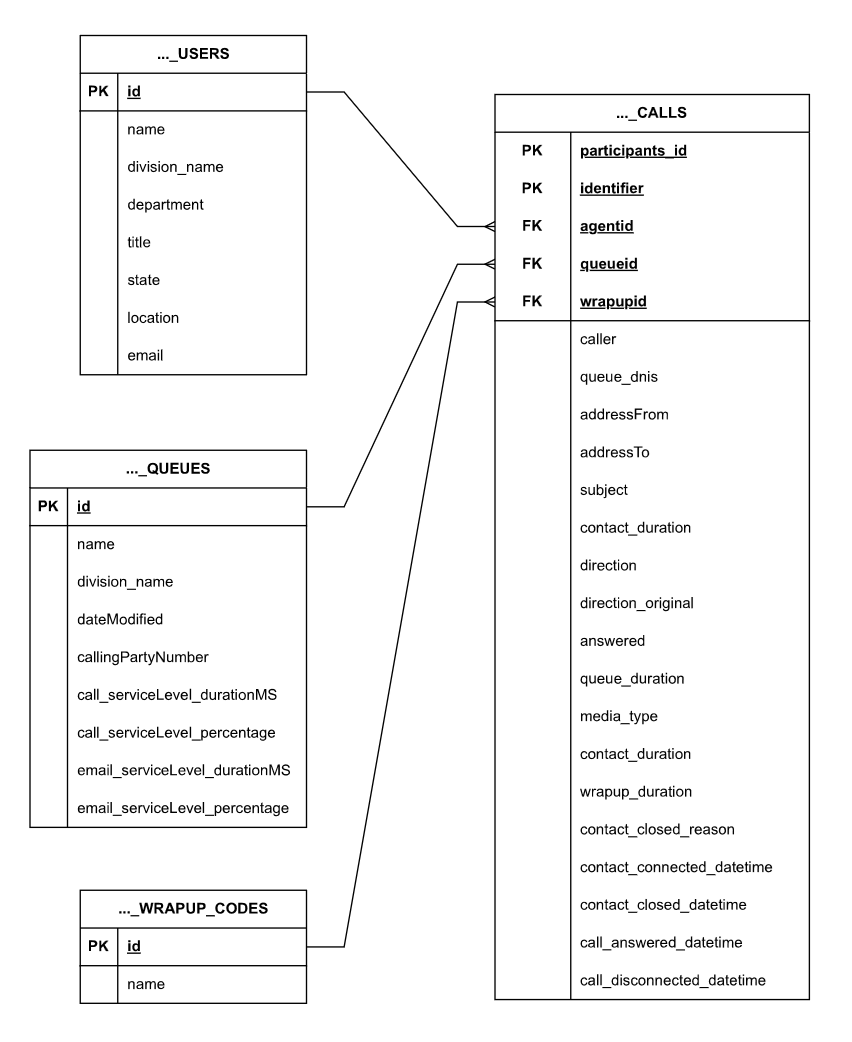
\includegraphics[width=1\textwidth]{media/table_spec.png}
  \caption{Tutkimuksessa käytettävän tietokannan rakenne.}
  \label{fig:table_spec}
\end{figure}

Tutkielman tavoitteena on arvioida, kuinka hyvin Cortex Analyst soveltuu luonnollisen kielen tietokantakyselyihin ja millaisia rajoituksia sen käyttöön liittyy. Koska nykyaikaisten kaupallisten kielimallien tarkat toteutustiedot eivät yleensä ole julkisia, järjestelmän arviointi perustuu empiiriseen tarkasteluun. Tässä työssä vertaillaan nimenomaan Cortex Analystin tuottamia SQL-kyselyitä eikä niiden palauttamia vastauksia. Rajaus on perusteltu sekä aineiston luottamuksellisuuden vuoksi että siksi, että virheellisen kyselyn vaikutus lopulliseen vastaukseen riippuu myös tietokannan sisällöstä.

tutkimust ohjaavat seuraavat tutkimuskysymykset: Kuinka konsistentisti Cortex Analyst tuottaa SQL-kyselyitä, kun sama kysymys esitetään useita kertoja? Kuinka herkkä Cortex Analyst on sellaisille syötteen muutoksille, joiden ei pitäisi muuttaa kysymyksen merkitystä? Millaisia virhe- ja vaihtelutyyppejä järjestelmän tuottamissa SQL-kyselyissä esiintyy?

Tutkielm etenee siten, että ensin kuvataan tutkimusasetelma, aineisto ja arviointitapa. Tämän jälkeen esitellään kokeet, joissa tarkastellaan järjestelmän konsistenssia ja herkkyyttä merkitykseltään vähäisille muutoksille. Lopuksi esitetään tulokset, johtopäätökset ja tutkimuksen keskeiset rajoitukset.

\section{Metodologia}

\subsection{Tutkimusasetelma}
Tutkimus toteutetaan empiirisenä tapaustutkimuksena, jossa arvioidaan yhden kielimallipohjaisen järjestelmän toimintaa rajatussa sovelluskontekstissa. Tavoitteena ei ole rakentaa uutta mallia tai vertailla useita eri järjestelmiä keskenään, vaan tarkastella, miten Cortex Analyst suoriutuu käytännöllisestä tehtävästä, jossa luonnollisen kielen kysymykset muunnetaan SQL-kyselyiksi. Tapaustutkimus soveltuu tähän tarkoitukseen hyvin, koska se mahdollistaa järjestelmän toiminnan yksityiskohtaisen tarkastelun todellisessa kaupallisessa ypmäristössä.

Tutkimuksen analyysiyksikkönä on yksittäinen käyttäjän luonnollisen kielen kysymys ja sitä vastaava Cortex Analystin tuottama SQL-kysely. Arviointi kohdistuu siihen, vastaako muodostettu kysely käyttäjän tarkoitusta, hyödyntääkö se oikeita tauluja ja kenttiä sekä noudattaako se tietokannan rakennetta. Näin tutkimus keskittyy suoraan siihen vaiheeseen, jossa kielimallin tulkinta muuttuu koneellisesti suoritettavaksi tietokantakyselyksi.

\subsection{Tutkimusaineisto}
Tutkimuksen aineistona toimii puhelinkeskusdataa sisältävä tietokanta. Tarkastelun keskiössä on yksi keskusteludataa sisältävä päätason taulu, jota täydentävät kolme liitännäistaulua. Liitännäistaulujen avulla voidaan tarkentaa päätason taulun yksittäisten kenttien sisältöä ja merkitystä. Tietokannan rakenne on siten riittävän monipuolinen, jotta voidaan tarkastella sekä yksinkertaisia että vaativampia kyselytilanteita, kuten taululiitoksia, suodatuksia ja aggregaatioita.

Aineisto sisältää kaupallisesti arkaluonteista tietoa, minkä vuoksi varsinaisia kyselytuloksia ei julkaista. Tästä syystä tutkimuksessa vertaillaan järjestelmän tuottamia SQL-kyselyitä eikä niiden palauttamia tietosisältöjä. Ratkaisu tukee myös analyysin johdonmukaisuutta, koska virheellisen kyselyn vaikutus lopputulokseen ei ole aina pääteltävissä pelkästään syntaksista, vaan riippuu osittain tietokannan sisällöstä.

\subsection{Cortex Analyst ja semanttinen näkymä}
Tutkimuksessa käytettävä järjestelmä on Snowflaken Cortex Analyst. Järjestelmän tarkoituksena on mahdollistaa tietokantatiedon hyödyntäminen luonnollisen kielen kautta siten, että käyttäjän ei tarvitse tuntea SQL-kieltä tai tietokannan skeemaa yksityiskohtaisesti. Cortex Analyst muodostaa käyttäjän kysymyksestä SQL-kyselyn ja voi suorittaa sen tietokantaa vasten.

Cortex Analystin toiminta perustuu semanttiseen näkymään, jossa tietokannan taulut, kentät ja niiden merkitykset kuvataan YAML-muotoisena määrittelynä (kts. kuva \ref{fig:example_semantic_view}). Semanttinen näkymä tarjoaa kielimallille rakenteellisen kuvauksen siitä, mitä tietoa tietokannassa on saatavilla ja miten eri taulut liittyvät toisiinsa. Näin järjestelmä pystyy muodostamaan syntaktisesti valideja SQL-kyselyitä ja kohdistamaan kyselyn oikeisiin tietokannan osiin. Semanttisen näkymän laatu on keskeinen osa järjestelmän toimivuutta, koska kielimallin tulkinta perustuu olennaisesti siihen, miten skeema on kuvattu.

\begin{figure}[h]
\begin{lstlisting}[language=yaml]
name: SEM_EXAMPLE
description: |-
  Semantic model that models conversations data from Genesys Cloud contact center software.
tables:
  - name: CONV
    description: |-
      All Genesys conversations.
    base_table:
      database: DEV
      schema: DBT_OM
      table: FACT_GENESYS__CONVERSATIONS_STANDARD
    dimensions:
      - name: C_ADDRESS_FROM
        description: Source address for the interaction. Only present in email contacts..
        expr: conv.address_from
        data_type: VARCHAR(16777216)
    facts:
      - name: CALL_DURATION
        description: Duration of the actual call in seconds. The time the customer speaks to an agent
        expr: conv.call_duration
        data_type: NUMBER(38,0)
        access_modifier: public_access
    metrics:
      - name: AVERAGE_CALL_DURATION
        description: Average call duration in seconds
        expr: sum(conv.call_duration)
        access_modifier: public_access
    primary_key:
      columns:
        - PARTICIPANTS_ID
        - IDENTIFIER
\end{lstlisting}
  \caption{Esimerkki semanttisesta näkymästä.}
  \label{fig:example_semantic_view}
\end{figure}

Cortex Analyst hyödyntää taustallaan Anthropicin Claude Sonnet 4 -mallia. Tästä seuraa, että tutkimuksen tulokset kuvaavat ensisijaisesti juuri tämän järjestelmän ja mallin yhdistelmän toimintaa. Tuloksia ei siksi voida sellaisenaan yleistää kaikkiin kielimalleihin tai muihin luonnollisen kielen tietokantarajapintoihin.

\subsection{Arviointiperusteet}
Tuotettuja SQL-kyselyitä arvioidaan useiden toisiaan täydentävien kriteerien avulla. Ensinnäkin tarkastellaan kyselyn syntaktista validiutta eli sitä, muodostuuko kyselystä teknisesti suorituskelpoinen SQL-lause. Toiseksi arvioidaan, valitseeko järjestelmä oikeat taulut ja käyttääkö se oikeita liitoksia silloin, kun käyttäjän kysymys edellyttää useamman taulun yhdistämistä. Kolmanneksi tarkastellaan suodatusehtoja, erityisesti where-lauseiden sisältöä, koska pienikin virhe niissä voi muuttaa kyselyn merkitystä olennaisesti. Lisäksi huomioidaan aggregaatiot, ryhmittelyt ja sarakevalinnat, jotta voidaan arvioida, vastaako kyselyn rakenne käyttäjän esittämää tiedontarvetta.

Arvioinnissa erotetaan toisistaan kaksi poikkeamatyyppiä. Ensimmäisessä tapauksessa SQL-kyselyt eroavat toisistaan syntaktisesti, mutta ovat sisällöllisesti käytännössä ekvivalentteja. Toisessa tapauksessa erot muuttavat kyselyn semanttista merkitystä, jolloin myös mahdollinen vastaus tietokannasta voisi muuttua. Tämä erottelu on tärkeä, koska puhtaasti syntaktiset erot eivät ole tutkimuskysymysten kannalta merkittäviä.

\section{Kokeet}
Ensimmäisessä kokeessa tarkastellaan Cortex Analystin konsistenssia, eli sitä, tuottaako järjestelmä saman SQL-kyselyn, kun sama luonnollisen kielen kysymys esitetään useita kertoja.

Toisessa kokeessa tarkastellaan järjestelmän herkkyyttä sellaisille syötteen muutoksille, joiden ei pitäisi muuttaa kysymyksen merkitystä. Näissä kokeissa muodostetaan useita eri sanamuotoja samasta tiedontarpeesta ja arvioidaan, tuottaako järjestelmä niistä olennaisesti saman SQL-kyselyn.

\paragraph{Konsistenssikoe}
Koska kielimallit ovat tilastollisia järjestelmiä, sama syöte ei välttämättä aina johda täsmälleen samaan tulosteeseen. Tietokantakyselyiden tapauksessa tämä on olennainen kysymys, koska käyttäjät odottavat järjestelmältä ennustettavaa ja toistettavaa toimintaa.

Konsistenssikokeessa sama luonnollisen kielen kysymys esitetään järjestelmälle 10 kertaa. Jokaisesta suorituksesta tallennetaan järjestelmän tuottama SQL-kysely, joita verrataan keskenään. Käytetyt kysymykset ovat seuraavat:
\begin{enumerate}[label=\Alph*.]\label{it:q_consistency}
  \item How many total contacts did we handle in January 2026?
  \item What's our answer rate for calls in February 2026?
  \item What percentage of contacts that were answered within our service level target were closed by the customer versus closed by the agent?
  \item What was our peak contact hours by day of week? Show me the distribution of when contacts arrive throughout the day, broken down by hour and weekday.
  \item What's the success rate of our callbacks? Show me how many callbacks resulted in a conversation versus no answer, and what the average time between the original inbound contact and the callback was.
\end{enumerate}

Määritellyssä semanttisessa näkymässä on kuvattu metriikoihin SQL-kyselyt, jotka vastaavat suoraan kysymyksiin 1 ja 2. Kysymykset 3-5 ovat huomattavasti monimutkaisempia, ja niihin ei ole ennalta validoituja SQL-kyselyitä semanttisessa näkymässä. Kysymys 4 vaatii, että kentästä \texttt{CONTACT\_CONNECTED\_DATETIME} erotetaan kellonaika tunnin tarkkuudella, ja viikonpäivä pitää hakea kalenteritaulusta. Kysymys 5 vaatii, että malli suodattaa takaisinsoitot oikein \texttt{direction\_original = 'inbound' AND direction = 'outbound'} -ehdon perusteella sekä osaa yhdistää takaisinsoiton vastaavaan alkuperäiseen soittoon.

\paragraph{Sensitiivisyyskoe}
Kokeen tavoitteena on arvioida, tulkitseeko Cortex Analyst semanttisesti saman sisältöiset kysymykset johdonmukaisesti vai johtavatko kielelliset erot erilaisiin SQL-kyselyihin. Jos järjestelmä on hyvin herkkä muotoilun vaihtelulle, luonnollisen kielen käyttö rajapintana muuttuu käyttäjän kannalta epävarmaksi. Jos taas järjestelmä tuottaa olennaisesti saman kyselyn eri sanamuodoista huolimatta, tämä tukee sen käytettävyyttä käytännön työssä.

Koe toteutetaan muodostamalla kustakin konsistenssikokeessa käytetystä kysymyksestä 4 vaihtoehtoista versiota, joissa pyritään säilyttämään kysymyksen merkitys, mutta muokkaamaan sanamuotoa. Järjestelmän tuottamat SQL-kyselyt tallennetaan ja vertaillaan keskenään. Käytetyt kysymykset ovat seuraavat:
\begin{enumerate}[label=\Alph*.]\label{it:q_sensitivity}
  \item Variaatioita kysymyksestä A:
    \begin{enumerate}[label=\arabic*.]
      \item What was the total number of contacts we handled in January 2026?
      \item How many contacts did we handle overall in January 2026?
      \item What is the total contact volume for January 2026?
      \item How many total customer contacts were handled during January 2026?
    \end{enumerate}
  \item Variaatioita kysymyksestä B:
    \begin{enumerate}[label=\arabic*.]
      \item What was our call answer rate in February 2026?
      \item What percentage of incoming calls were answered in February 2026?
      \item What percentage of calls were answered in February 2026?
      \item How did our call answer rate perform during February 2026?
    \end{enumerate}
  \item Variaatioita kysymyksestä C:
    \begin{enumerate}[label=\arabic*.]
      \item Of the contacts answered within our service-level target, what share were closed by the customer compared to those closed by the agent?
      \item For interactions resolved within the service level target, what percentage were customer-closed versus agent-closed?
      \item Within our service level target, how is the closure split: what percent of contacts were closed by customers versus agents?
      \item Among contacts answered within SLA, what proportion ended with customer closure versus agent closure?
    \end{enumerate}
  \item Variaatioita kysymyksestä D:
    \begin{enumerate}[label=\arabic*.]
      \item For each weekday, what were our peak contact hours, and how are contacts distributed across the day (by hour)?
      \item Show the hourly contact-arrival distribution for every day of the week, highlighting which hours were highest on each weekday.
      \item What times during the day (hour-by-hour) drive the most contacts, split by weekday. Please summarize peak hours and the overall distribution.
      \item Across the week, when do contacts arrive most often? Provide an hour-by-hour breakdown for each weekday and identify the peak contact hours.
    \end{enumerate}
  \item Variaatioita kysymyksestä E:
    \begin{enumerate}[label=\arabic*.]
      \item What percentage of our callback attempts lead to an actual conversation? Please break down callbacks that reached a conversation vs. those with no answer, and calculate the average delay from the original inbound to the callback.
      \item How effective are our callbacks? Show the success rate by counting callbacks that resulted in a conversation versus no answer, and report the average time-to-callback from the initial inbound contact.
      \item For our callback campaign, what's the outcomes split and average response speed? Provide counts of conversations vs. no-answer callbacks, the resulting success rate, and the average elapsed time between inbound contact and callback.
      \item Can you analyze callback performance for me: success rate (conversation vs no answer) with the number of callbacks in each outcome category, plus the average time lag from the inbound contact to when the callback occurred?
    \end{enumerate}
\end{enumerate}

\subsection{Kyselyiden vertailu ja luokittelu}
Molempien kokeiden tuottamat SQL-kyselyt analysoidaan systemaattisesti. Kysleyt luokitellaan korrektiksi, jos ne ovat semanttisesti ekvivalentteja halutun kyselyn kanssa, vaikka ne eivät olisikaan merkkijonotasolla identtisiä. Kyselyt luokitellaan virheellisiksi, jos ne eivät ole semanttisesti ekvivalentteja halutun kyselyn kanssa.

\section{Tulokset}
Merkitään konsistenssikokeen kysymykset A-E ja herkkyyskokeen variaatiot A1-A4, B1-B4, C1-C4, D1-D4 ja E1-E4. Kokeiden tulokset on esitetty taulukoissa \ref{tb:consistency}, \ref{tb:sensitivity1}, \ref{tb:sensitivity2}, \ref{tb:sensitivity3}, \ref{tb:sensitivity4} ja \ref{tb:sensitivity5}. Taulukot kuvaavat kunkin kysymyksen osalta sitä, kuinka monta kertaa järjestelmä tuotti semanttisesti korrektin SQL-kyselyn, kuinka monta kertaa kysely oli buginen (eli syntaktisesti virheellinen) ja kuinka monta kertaa kysely oli väärin (eli semanttisesti virheellinen).

Lisäksi konsistenssikokeen taulukossa on sarake uniikkien SQL-kyselyiden määrästä, joka kuvaa, kuinka monella eri tavalla järjestelmä muotoili SQL-kyselyn kyseiselle luonnollisen kielen kysymykselle. Herkkyyskokeen taulukoissa ollaan listattu kumulatiivinen uniikkien SQL-kyselyiden määrä, koska niissä tarkastellaan nimenomaan sitä, tuottaako järjestelmä saman SQL-kyselyn eri variaatioista.

\renewcommand{\arraystretch}{1.25}
\begin{table}[ht]
  \centering
  \caption{Konsistenssikokeen tulokset. Jokainen kysymys (kts. lista \ref{it:q_consistency}) esitettiin 10 kertaa, ja taulukkoon on koottu jakauma siitä, kuinka monta kertaa järjestelmä tuotti semanttisesti korrektin SQL-kyselyn.}
  \label{tab:results}
  \small
  \begin{tabular}{ccccc}\label{tb:consistency}
    \toprule
    Kysymys & Korrekti & Buginen & Väärin & Uniikkien SQL-kyselyiden määrä \\
    \midrule
    A & 10 & 0 & 0 & 1\\
    B & 10 & 0 & 0 & 2 \\
    C & 7 & 0 & 3 & 2\\
    D & 0 & 10 & 0 & 1\\
    E & 0 & 0 & 10 & 1\\
    \bottomrule
  \end{tabular}

\end{table}

\begin{table}[ht]\label{tb:sensitivity1}
  \centering
  \caption{Herkkyystestin 1 tulokset. Jokainen kysymys esitettiin 10 kertaa, ja taulukkoon on koottu jakauma siitä, kuinka monta kertaa järjestelmä tuotti semanttisesti korrektin SQL-kyselyn.}
  \small
  \begin{tabular}{ccccc}
    \toprule
    Kysymys & Korrekti & Buginen & Väärin & Uniikkien SQL-kyselyiden määrä \\
    \midrule
    A & 10 & 0 & 0 & 1\\
    A1 & 10 & 0 & 0 & 1\\
    A2 & 10 & 0 & 0 & 1 \\
    A3 & 10 & 0 & 0 & 1\\
    A4 & 0 & 10 & 0 & 1\\
    \bottomrule
  \end{tabular}
\end{table}

\begin{table}[ht]\label{tb:sensitivity3}
  \centering
  \caption{Herkkyystestin 3 tulokset. Jokainen kysymys esitettiin 10 kertaa, ja taulukkoon on koottu jakauma siitä, kuinka monta kertaa järjestelmä tuotti semanttisesti korrektin SQL-kyselyn.}
  \small
  \begin{tabular}{ccccc}
    \toprule
    Kysymys & Korrekti & Buginen & Väärin & Uniikkien SQL-kyselyiden määrä \\
    \midrule
    C & 7 & 0 & 3 & 2\\
    C1 & 8 & 0 & 2 & 2\\
    C2 & 10 & 0 & 0 & 1 \\
    C3 & 0 & 0 & 10 & 2\\
    C4 & 8 & 0 & 2 & 4\\
    \bottomrule
  \end{tabular}
\end{table}

\begin{table}[ht]\label{tb:sensitivity4}
  \centering
  \caption{Herkkyystestin 4 tulokset. Jokainen kysymys esitettiin 10 kertaa, ja taulukkoon on koottu jakauma siitä, kuinka monta kertaa järjestelmä tuotti semanttisesti korrektin SQL-kyselyn.}
  \small
  \begin{tabular}{ccccc}
    \toprule
    Kysymys & Korrekti & Buginen & Väärin & Uniikkien SQL-kyselyiden määrä \\
    \midrule
    D & 0 & 10 & 0 & 1\\
    D1 & 0 & 0 & 10 & 2\\
    D2 & 10 & 0 & 0 & 1 \\
    D3 & 0 & 0 & 10 & 2\\
    D4 & 0 & 0 & 10 & 2\\
    \bottomrule
  \end{tabular}
\end{table}

\begin{table}[ht]\label{tb:sensitivity5}
  \centering
  \caption{Herkkyystestin 5 tulokset. Jokainen kysymys esitettiin 10 kertaa, ja taulukkoon on koottu jakauma siitä, kuinka monta kertaa järjestelmä tuotti semanttisesti korrektin SQL-kyselyn.}
  \small
  \begin{tabular}{ccccc}
    \toprule
    Kysymys & Korrekti & Buginen & Väärin & Uniikkien SQL-kyselyiden määrä \\
    \midrule
    E & 0 & 0 & 10 & 1\\
    E1 & 0 & 0 & 10 & 1\\
    E2 & 0 & 0 & 10 & 2 \\
    E3 & 0 & 0 & 10 & 1\\
    E4 & 0 & 0 & 10 & 1\\
    \bottomrule
  \end{tabular}
\end{table}

\section{Rajoitukset}
Tutkimukseen liittyy useita rajoituksia, jotka on huomioitava tuloksia tulkittaessa. Ensinnäkin tutkimus kohdistuu yhteen järjestelmään, Snowflaken Cortex Analystiin, jonka taustalla toimii Anthropicin Claude Sonnet 4 -malli. Tulokset kuvaavat siis yhtä tiettyä toteutusta eivätkä ole suoraan yleistettävissä muihin kielimalleihin, SQL-avustajiin tai luonnollisen kielen analytiikkatyökaluihin.

Toiseksi tutkimus perustuu yhteen sovellusalueeseen eli puhelinkeskusdataan. Tämän tietokannan rakenne, sanasto ja analyysitarpeet voivat poiketa merkittävästi muiden toimialojen vastaavista ympäristöistä. On mahdollista, että järjestelmä suoriutuisi eri tavalla esimerkiksi talousdatan, lokidatan tai asiakastietojen yhteydessä.

Kolmanneksi tutkimuksessa tarkastellaan mallin tuottamia SQL-kyselyitä eikä kyselyiden palauttamia varsinaisia vastauksia. Tämä rajaus on perusteltu aineiston luottamuksellisuuden vuoksi, mutta samalla se tarkoittaa, että tutkimus ei suoraan mittaa liiketoiminnallisen lopputuloksen oikeellisuutta. Kysely voi olla rakenteeltaan puutteellinen tai vaihtoehtoisesti syntaktisesti erilainen mutta käytännössä toimiva, eikä tätä eroa voida aina arvioida täysin ilman varsinaista tulosaineistoa.

Neljänneksi semanttisen näkymän laatu vaikuttaa suoraan siihen, miten hyvin Cortex Analyst kykenee muodostamaan kyselyitä. Jos näkymässä on epäselvyyksiä, puutteita tai monitulkintaisia kuvauksia, osa havaituista ongelmista voi johtua itse määrittelystä eikä pelkästään kielimallin rajoituksista. Tämän vuoksi tutkimus arvioi samalla myös sitä, kuinka hyvin kyseinen semanttinen näkymä tukee luonnollisen kielen ja tietokantarakenteen välistä tulkintaa.

Viidenneksi kielimallien toimintaa luonnehtii tietty epädeterministisyys, minkä vuoksi tulokset voivat vaihdella eri suorituskerroilla tai järjestelmäversioiden välillä. Tästä syystä tutkimuksen havainnot kuvaavat järjestelmän toimintaa tiettynä ajankohtana ja tietyssä konfiguraatiossa, eivät välttämättä pysyvää ominaisuutta.
